\documentclass[10pt,a4paper]{amsart}
\usepackage[margin=19mm]{geometry}
\usepackage{amsmath,amssymb,mathtools}
\usepackage[scr=rsfs,cal=euler]{mathalfa}
\usepackage{xfrac}
\usepackage[unicode,hidelinks,bookmarks=false]{hyperref}
\newcommand{\ie}{i.e.\ }
\newcommand{\cf}{cf.\ }
\newcommand{\resp}{respectively\ }
\newcommand{\Subsection}{\subsection}
\providecommand{\nobreakdash}{\nobreak\hbox{-}}
\setlength{\emergencystretch}{2em}
\multlinegap0pt
\usepackage{dsfont}
\usepackage{tikz}
\usepackage{caption}
\numberwithin{equation}{section}
\DeclareMathOperator{\R}{\mathbb{R}}
\DeclareMathOperator{\N}{\mathbb{N}}
\DeclareMathOperator{\Q}{\mathbb{Q}}
\DeclareMathOperator{\T}{\mathbb{T}}
\DeclareMathOperator{\Var}{Var}
\newcommand{\bbN}{\mathbb{N}}
\newcommand{\bbT}{\mathbb{T}}
\newcommand{\bbP}{\mathbb{P}}
\newcommand{\bbR}{\mathbb{R}}
\newcommand{\rmd}{\mathrm{d}}
\newcommand{\bbQ}{\mathbb{Q}}
\newcommand{\bbZ}{\mathbb{Z}}
\newcommand{\clE}{\mathcal{E}}
\newcommand{\clA}{\mathcal{A}}

%\newcommand{\ql}{q_{\ell}}
\newcommand{\yn}{(y_n)_{n\,\in\,\mathbb{N}} }
\newcommand{\kj}{n_{\ell}}
\newcommand*{\mk}{\mkern -1mu}
\newcommand*{\Mk}{\mkern -2mu}
\newcommand*{\mK}{\mkern 1mu}
\newcommand*{\MK}{\mkern 2mu}
\let\oldtilde\tilde
\renewcommand*{\tilde}[1]{\mathchoice{\widetilde{#1}}{\widetilde{#1}}{\oldtilde{#1}}{\oldtilde{#1}}}
\let\oldforall\forall
\renewcommand*{\forall}{\mathrel{\oldforall}}
\newtheorem{theo}{Theorem}[section]
\newtheorem{prop}[theo]{Proposition}
\newtheorem{lemm}[theo]{Lemma}
\theoremstyle{definition}
\newtheorem{defi}[theo]{Definition}
\newtheorem{rema}[theo]{Remark}
\title[No temporal distributional limit for finite sawtooth--step sums]{Absence of nondegenerate temporal limit laws for finite sawtooth--step sums with a nonzero jump, almost every circle rotation and every starting point}
\author{Lorenz Fr\"uhwirth and Manuel Hauke}
\date{Source: Annales Henri Lebesgue \textbf{7} (2024), 251--265; DOI 10.5802/ahl.200; official published version}
\begin{document}
\maketitle
\noindent\textit{Editorial scope.} The counted unit is original Theorem 1.2 with its complete authored proof. Retained uncounted core: the original definition of a piecewise smooth function, the original definition of a temporal distributional limit theorem, the paper's own continued-fraction and Koksma prerequisites, and Propositions 3.1--3.3, Lemma 3.4, Remark 3.5, Proposition 3.6 and Lemma 3.7 with their complete proofs, all copied exactly from the publisher-native source. All hypotheses, constants, theorem and equation numbers and citation labels are those of the published version; the paper's later applications to the question of Dolgopyat and Sarig are not selected. Literal print slips inside the retained text are kept without mathematical repair and are recorded in the scope note of the manifest.
\section{Introduction and main results}

Let $X$ be a metric space, $T : X \to X$ a Borel measurable map, $f: X \to \R$ a measurable function and $x_0 \in X$. Then
\[
S_N(f,T,x_0) = \sum_{k=0}^{N-1} f \circ T^k(x_0)
\]
defines the Birkhoff sum of $f$ over $T$ at stage $N$ with starting point $x_0$. A pair $(T,f)$ is said to satisfy a temporal distributional limit theorem (TDLT) along the orbit of a fixed $x_0 \in X$ whenever there exist two sequences $(A_M(f,T,x_0))_{M\,\in\,\bbN}$, $(B_M(f,T,x_0))_{M\,\in\,\bbN}$ with $\lim_{M\,\to\,\infty} B_M = \infty$, and a non-constant random variable $Y$ such that
\begin{equation}\label{TLT}
\lim_{M\,\to\,\infty} \frac{1}{M} \# \left\{1 \leq N \leq M: \frac{S_N(f,T,x_0) - A_M}{B_M} \leq a\right\} = \bbP[Y \leq a].
\end{equation}

\begin{defi}[Piecewise smooth functions]\label{def_fct1}
We call a function $f: \bbT \to \bbR$ with $\int_{\bbT} f(x)\,\rmd  \mu(x) = 0$ a \emph{piecewise smooth function} if there exist $ \nu \geq 1$ and $ \{\gamma_1,\,\ldots,\,\gamma_\nu \} \subseteq \T$ with $ 0 \leq \iota(\gamma_1) < \ldots < \iota(\gamma_{ \nu}) < 1$ ($\iota$ denotes the canonical embedding $\T \hookrightarrow [0,1)$, see Section~\ref{Sec_preReq}) such that the following properties hold:
\begin{itemize}
\item $f$ is differentiable on $\bbT\setminus \{\gamma_1,\,\ldots,\,\gamma_{\nu}\}$.
\item $f'$ extends to a function of bounded variation on $\bbT$.
\item There exists an $i \in \{1,\,\ldots,\,\nu\}$ such that $\lim_{ \delta \rightarrow 0} [f(\gamma_i - \delta) - f(\gamma_i+ \delta)] \neq 0$.
\end{itemize}
\end{defi}

\setcounter{theo}{1}
\begin{theo}\label{thm_no_LT}
Let $f$ be a piecewise smooth function (see Definition~\ref{def_fct1}). Then for (Haar-) almost all $ \alpha \in \bbT$ and for any $x_0 \in \T$ the following holds: Let $N$ be uniformly distributed on $\{1,\,\ldots,\,M\}$. Then the sequence of random variables $(\frac{S_{N}(f,T_{\alpha},x_0) - A_M}{B_M})_{M\,\in\,\bbN}$ does not satisfy a distributional limit theorem in the sense of~\eqref{TLT}, regardless of how $(B_M)_{M\,\in\,\N}$ and $(A_M)_{M\,\in\,\N}$ are chosen.
\end{theo}

\section{Prerequisites}\label{Sec_preReq}

\subsection*{Notation}

Given two functions $f,g:(0,\infty)\to \bbR,$ we write $f(t) = O(g(t)), f \ll g$ or $g \gg f$ if $\limsup_{t\,\to\,\infty} \frac{|f(t)|}{|g(t)|} < \infty$. Any dependence of the value of the limes superior above on potential parameters is denoted by appropriate subscripts. For two sequences $ (a_k)_{k\,\in\,\N}$ and $(b_k)_{k \,\in\,\N}$ with $b_k \neq 0$ for all $k \in \N$, we write $a_k \sim b_k, k \to \infty$, if $ \lim_{k \to \infty} \frac{a_k}{b_k}=1$. We denote the characteristic function of a set $A$ by $\mathds{1}_A$ and understand the value of empty sums as $0$. For $A \subseteq \N$, we define the lower density of $A$ as $\liminf\limits_{N\,\to\,\infty}\frac{1}{N} \# (A \cap [\![1,N]\!])$.

\noindent To avoid confusion between elements on $\T \simeq {\Large{\sfrac{\R}{\bbZ}}}$ and on $\R$, we use the following notation: We write $\iota: \T \hookrightarrow [0,1)$ for the canonical embedding. Given a real number $\alpha$, we denote its fractional part as $\{ \alpha \} := \alpha - \lfloor \alpha \rfloor $. Further, let $\| x \| := \min\{\iota(x),1 - \iota(x)\}$ denote the canonical norm on $\T$. We will denote the normalized Haar measure on $\T$ by $\mu$. For $a,b,x \in \T$, we understand $ \mathds{1}_{[a,b]}(x) $ as $ \mathds{1}_{[\iota(a),\iota(b)]}(\iota(x))$. For $a \in \T$ and $n \in \N$, we define as usual $na :=\sum_{i=1}^n a$. If $x \in \R$ and $a \in \T$, we understand $x + a $ as $\iota^{-1}(x) + a \in \T $.

Let $X,Y$ be two real-valued random variables defined on a common probability space. If $X$ and $Y$ have the same distribution, we write $X \stackrel{d}{=} Y$. If $X$ has the distribution $\mu$ we write $X \sim \mu$. Let $A,B$ be two events on a common probability space with probability measure $\bbP$, then $\bbP [A|B] := \frac{ \bbP[A \cap B]}{\bbP [B]} $ denotes the conditional probability of $A$ given $B$. For $a,b \in \R$ with $a<b$, we denote the uniform distribution on $[a,b]$ as $U([a,b])$. When $a,b \in \N_0$ with $a < b$, $U([\![a,b]\!])$ is the (discrete) uniform distribution on $[a,b] \cap \N_0$.

\subsection*{Continued fractions and Koksma's inequality}\label{cf_prop}


In this subsection, we recall several well-known results from the theory of continued fractions which are heavily used in the proof of Theorem~\ref{thm_no_LT}. For a more detailed background, we refer the reader to classical literature such as~\cite{all_shall,rock_sz}. Every irrational $\alpha \in [0,1)$ has a unique infinite continued fraction expansion denoted by $[0;a_1,a_2,\dots]$ with convergents $p_k/q_k := [0;a_1,\,\dots,\,a_k]$ that satisfy the recursions
\begin{equation*}
p_{k+1} = p_{k+1}(\alpha) = a_{k+1}(\alpha) p_k + p_{k-1}, \qquad q_{k+1} = q_{k+1}(\alpha) = a_{k+1}(\alpha) q_k + q_{k-1}, \quad k \in \N,
\end{equation*}
with initial values $p_0 = 0,\; p_1 = 1,\; q_0 = 1,\; q_1 = a_1$. For the sake of brevity, we just write $a_k, p_k, q_k$, although these quantities depend on $\alpha$. Note that the convergents $p_k/q_k$ satisfy the inequalities

\begin{equation}\label{Eq_parity_deltak}
\frac{1}{(a_{k+1} +2)q_{k}} \leq \delta_k := (-1)^k (q_k \alpha - p_k) \leq
\frac{1}{a_{k+1}q_k}, \quad k \geq 1.
\end{equation}

Conversely, if $| \alpha - p/q| < \frac{1}{2q^2}$, Legendre's Theorem implies that $p/q$ is a convergent of $\alpha$.

Since this article deals with almost sure behaviour, we also make use of the following classical results that arise from the well-studied area of the \emph{metric} theory of continued fractions:
\begin{itemize}
\item (Diamond and Vaaler~\cite{diamond_vaaler}): For almost every $\alpha$,
\begin{equation}\label{Eq_trimmed_sum}
\sum_{\ell\,\leq\,K} a_{\ell} - \max\limits_{\ell\,\leq\,K} a_{\ell} \sim \frac{K \log K}{\log 2}, \quad K \to \infty.
\end{equation}
\item (Khintchine and Lévy, see, e.g., \cite[Chapter~5, \S9, Theorem~1]{rock_sz}): For almost every $\alpha$,
\begin{equation}\label{Eq_size_of_q_k}
\log q_k \sim \frac{\pi^2}{12 \log 2} k, \quad k \to \infty.
\end{equation}
\end{itemize}

On several positions in the proof, we will make use of Koksma's inequality which allows to estimate the error between sums and corresponding integrals. For more details about this topic and the closely related area of Discrepancy theory, we refer the reader to~\cite{kuipers}. Denoting the discrepancy of a sequence $\yn \subseteq \T$ at stage $N \in \N$ by
\[
D_N(\yn) := \sup\limits_{0\,\leq\,a\,\leq\,b\,<\,1} \left | \frac{1}{N}\#\left\{1 \leq n \leq N: \iota(y_n) \in [a,b]\right\} - (b-a) \right |
\]
and the total variation of $f: \T \to \R$ by $\Var(f)$, Koksma's inequality is given by
\[
\left| \sum_{i=1}^{N} f(y_i) - N\int_{\T} f(x) \rmd \mu(x) \right| \leq \Var(f)N D_N(\yn).
\]

In the special case where $\yn$ is the Kronecker sequence $(n\alpha)_{n\,\in\,\N}$, we have the estimates
\[
D_{q_n}(\yn) \ll \frac{1}{q_n}, \quad D_{N}(\yn) \ll \frac{1}{N}\sum_{i=1}^{k} a_i,
\]
where $k = k(N)$ is such that $q_{k-1} \leq N < q_{k}$. Thus Koksma's inequality leads (in this particular case also known as Denjoy-Koksma inequality, see, e.g., \cite{herman}) to
\begin{equation}\label{denj_koks}
\left | S_{q_n}(f, \alpha, x_0) \right |
\ll_f 1, \quad
\left | S_{N}(f, \alpha, x_0) \right | \ll_f \sum_{i=1}^{k} a_i,
\end{equation}
with the implied constant being uniform in $x_0$.

\section{Proof of Theorem~\ref{thm_no_LT}}\label{Sect_Pf_noCLT}
\subsection{Preparatory Lemmas}\label{Sec_prepLemmas}

\begin{prop}\label{LemRepresentationf}
Let $f : \T \rightarrow \R$ be as in Definition~\ref{def_fct1}. Let $h:\T \to \R$ be defined as
\[
h(x) = \sum_{i=1}^{\nu} H_i\left (\iota(x) - \frac{1}{2} \right) + \sum_{i=1}^{\nu} H_i \left(\mathds{1}_{[0, \gamma_i)}(x) -\iota(\gamma_i) \right),
\]
where $H_i := \lim_{\delta\,\rightarrow\,0} [f(\gamma_i - \delta) - f(\gamma_i + \delta)]$. Then, for almost every $\alpha \in \T$, any $N \in \N$ and any $y \in \T$, we have
\[
S_N(f,\alpha,y) = S_N(h,\alpha,y) + O_{f, \alpha}(1),
\]
with the implied constant only depending on $f$ and $\alpha$.
\end{prop}

\begin{proof}
This can be proven analogously to~\cite[Lemma~3.1]{upper_dens}. A more detailed proof can be found in~\cite[Appendix~A]{quenched}.
\end{proof}

\begin{prop}\label{ds_thm}
(Duffin and Schaeffer, \cite[Theorem~3]{duff_sch}).
Let $A \subseteq \N$ be a set of positive lower density and $\psi: \N \to [0,\infty)$ be a monotone decreasing function such that $\sum_{q =1}^{\infty} \psi(q) = \infty$. Then, for almost every $\alpha$, there exist infinitely many coprime $(p,q) \in \bbZ \times A$ that satisfy $| \alpha - \frac{p}{q}| < \frac{\psi(q)}{q}$.
\end{prop}

\begin{prop}[{Cassels~\cite[Lemma~9]{cassels}}]\label{gallagher}
Let $(I_k)_{k\,\in\,\N} \subseteq \T$ be a sequence of intervals with $\lim_{k\,\to\,\infty} \mu(I_k) = 0$. Further let $c > 0$ and $(U_k)_{k\,\in\,\N}$ be a sequence of measurable sets that satisfy the following for all $k \in \N$:
\begin{itemize}
\item $U_k \subseteq I_k$,
\item $\mu(U_k) \geq c \mu(I_k)$.
\end{itemize}
Then, $\mu(\limsup\limits_{k\,\to\,\infty} U_k) = \mu(\limsup\limits_{k\,\to\,\infty} I_k)$.
\end{prop}


Combining the statements above, we can deduce the following result.

\begin{lemm}\label{Lem_seq_kj}
Let $A \subseteq \N$ be a set with positive lower density. Then, for almost every $\alpha = [0;a_1, a_2,\,\ldots] \in \T$, there exists a sequence of even integers $(k_j)_{j\,\in\,\N}$ such that $q_{k_j} \in A$ for all $j \in \N$ and $ \lim_{j\,\to\,\infty} \frac{\sum_{i=1}^{k_j} a_i }{a_{k_j +1}} = 0$.
\end{lemm}


\begin{proof}
Let $ \psi(q) = \frac{1}{q \log q \log \log q \log \log \log q }$\footnote{For convenience, we set $ \log x := 1$ if $x \leq e$.}, then it holds that $ \sum_{q\,\in\,\N} \psi(q)= \infty$ as well as $\psi(q) \leq 1$ for all $q \in \N$.


Let $(r_k/s_k)_{k\,\in\,\N}$ be the set of rationals with $s_k \in A$ and $1 \leq r_k \leq s_{k}-1$ with $\gcd(r_k,s_k) =1$. We define
\begin{equation*}
I_k:= \iota^{-1}\left(\frac{r_k}{s_k} - \frac{\psi(s_k)}{s_k}, \frac{r_k}{s_k} + \frac{\psi(s_k)}{s_k} \right) \quad \text{and} \quad U_k := \iota^{-1}\left(\frac{r_k}{s_k}, \frac{r_k}{s_k} + \frac{\psi(s_k)}{s_k} \right).
\end{equation*}
By Proposition~\ref{ds_thm}, we have $\mu(\limsup_{k\,\to\,\infty} I_k) = 1$. Since clearly $U_k \subseteq I_k$ and $ \mu(U_k) \geq \frac{1}{2}\mu(I_k)$ for all $k \in \N$, an application of Proposition~\ref{gallagher} shows \newline$ \mu(\limsup_{k\,\rightarrow\,\infty} U_k)  = 1$. In other words, for almost all $\alpha \in \T$, there are infinitely many coprime pairs $(p,q) \in \N \times A$ such that
\begin{equation}\label{EqApproxpq}
0 \leq \alpha - \frac{p}{q} < \frac{\psi(q)}{q} = \frac{1}{q^2 \log q \log \log q \log \log \log q}.
\end{equation}
By Legendre's Theorem, for $q \geq 10$, the above is only possible if $ (p,q)$ is a convergent of $\alpha $. Thus, the pairs $(p,q), q \geq 10$ that satisfy~\eqref{EqApproxpq} form a subsequence $ (p_{k_j}, q_{k_j})_{j\,\in\,\N}$ of the sequence of convergents $ (p_k, q_k)_{k\,\in\,\N}$. Since $\alpha - \frac{p_{k_j}}{q_{k_j}} \geq 0 $ for all $j \in \N$, it follows by~\eqref{Eq_parity_deltak} that all $k_j$ are even. Moreover, by construction of $\psi$ and combining~\eqref{Eq_parity_deltak} and~\eqref{Eq_size_of_q_k}, we have $ a_{k_j+1} \gg k_j \log k_j \log \log k_j$. By~\eqref{Eq_trimmed_sum} this implies that for almost every $\alpha$, we have $\sum_{i=1}^{k_j} a_i = o (a_{k_j +1}) $.
\end{proof}

\begin{rema}\label{Rem_evenoddIndices}
By obvious modifications, the statement of Lemma~\ref{Lem_seq_kj} also holds when ``even'' is replaced by ``odd''. In Lemma~\ref{indicator_lem}, this would lead to an even larger class of limiting distributions that are realized as limits of certain Birkhoff sums along suitable subsequences. For our purpose of ruling out any TDLT, the stated version of Lemma~\ref{Lem_seq_kj} is sufficient.
\end{rema}



\begin{prop}\label{isolated_density}
Let $\beta_1,\beta_2,\,\ldots,\,\beta_{\nu} \in \T \setminus \{0\}, \nu \in \N$. Then there exists $\delta> 0$ such that the set $\{N \in \N: \forall 1 \leq j \leq \nu: \| N\beta_j \| > \delta \}$ has positive lower density.
\end{prop}

\begin{proof}
We partition $\{ \beta_i \}_{i=1}^{\nu} $ into rational and irrational numbers. Without loss of generality, we may assume $\iota(\beta_1) = \frac{a_1}{b_1},\,\ldots,\,\iota(\beta_k) = \frac{a_k}{b_k} \in \Q$ with $a_i,b_i \in \N, \gcd(a_i,b_i) = 1, b_i \geq 2$ since $\beta_i \neq 0$ for $i = 1,\,\ldots,\,k$, and $\iota(\beta_{k+1}),\ldots,\iota(\beta_{\nu}) \notin \Q$. Let $b_{\pi} := \prod_{i=1}^{k}b_i$. Clearly, if $N \equiv 1 \pmod {b_{\pi}}$, then for all $1 \leq i \leq k$, $b_i \nmid N$ and thus, $\iota(N\beta_i) \in \{\frac{1}{b_i},\,\ldots,\,\tfrac{b_i-1}{b_i}\}$, which is disjoint from $(0,\delta) \cup (1-\delta,1)$ if $\delta$ is chosen sufficiently small. Since $\{N \in \N: N \equiv 1 \pmod{b_{\pi}}\}$ has positive lower density, it suffices to show that
\begin{equation*}
\left\{M \in \bbN: \forall i \in \{k+1,\ldots,\nu\}:
\| (M b_{\pi}+1)\beta_i \| > \delta \right\}
\end{equation*}
has positive lower density. Since $ \iota (b_{\pi} \beta_i) \notin \Q$ for all $i=k+1,\,\ldots,\,\nu$, it follows that $ \left \{ (M b_{\pi} \beta_i + \beta_i)\right\}_{M\,\in\,\N}$ is uniformly distributed on $\T$. This immediately shows
\[
\liminf_{N\,\to\,\infty}
\frac{1}{N}\#\left\{M \leq N: \forall i \in \{k+1,\,\ldots,\,\nu\}:
\| (M b_{\pi}+1)\beta_i \| > \delta \right\}
\geq 1 - 2\nu\delta > 0,
\]
provided $\delta < \frac{1}{2\nu}$.
\end{proof}

\subsection{Main Lemma and conclusion of the proof}\label{SubSec_proofThm}

\begin{lemm}\label{indicator_lem}
Let $f(x) =(\sum_{i=1}^{\nu} H_i) (\iota(x) - \frac{1}{2}) + \sum_{i=1}^{\nu} H_i (\mathds{1}_{[0, \gamma_i)} (x) - \iota(\gamma_i))$ where $\gamma_1,\,\ldots,\,\gamma_{\nu} \in \bbT$ are distinct. Then for almost every $\alpha = [0;a_1,a_2,\,\ldots] \in \T$ and any $x_0 \in \T$, there exists an increasing sequence $({\kj})_{\ell\,\in\,\N}$ such that the following holds:
\begin{itemize}
\item For every $\ell \in \N$, $q_{\kj}$ is a denominator of a convergent of $\alpha$.
\item $\lim_{\ell\,\to\,\infty} \frac{\sum_{i =1}^{\kj} a_i }{a_{\kj+1}} = 0$.
\item The limits
\[
\overline{x_0} := \lim_{\ell\,\to\,\infty} q_{\kj}x_0, \quad \overline{\gamma_i} := \lim_{\ell\,\to\,\infty} q_{\kj}\gamma_i, \quad i = 1,\,\ldots,\,\nu \quad
\]
exist and satisfy $\overline{\gamma_i} \neq \overline{\gamma_1}$ for all $i = 2,\,\ldots,\,\nu$. If $\gamma_1 \neq 0$, then $\overline{\gamma_1} \neq 0$.
\item We have
\begin{multline}\label{def_of_g}
\lim_{\ell\,\to\,\infty}
\sup_{c\,\in\,[0,1]} \left\vert
\frac{S_{ \lfloor c a_{\kj+1}\rfloor q_{\kj} }(f,\alpha,x_0)}{a_{\kj+1}}\right. \\
-\left. \left(\left(\sum_{i = 1}^{\nu} H_i \right) \left(\int_{0}^{c} \iota(y + \overline{x_0}) \, \rmd y - \frac{c}{2}\right) 
+ \sum_{i = 1}^{\nu} H_i\left(\int_{0}^{c} \mathds{1}_{\left[0, \overline{\gamma_i}\right]}\left(y + \overline{x_0}\right) \,\rmd y - \iota(c\overline{\gamma_i})\right)\right)\right\vert = 0.
\end{multline}
\end{itemize}
\end{lemm}

\begin{proof}
Without loss of generality, we may assume that $\gamma_i \neq 0$ for all $i = 1,\,\ldots\nu$, since otherwise, we observe that $S_N(f,\alpha,x_0) = S_N(\tilde{f},\alpha,x_0 + y_0)$ where $\tilde{f}(x) = f(x- y_0)$ and $y_0$ is chosen such that $\gamma_i + y_0 \neq 0$ for all $i = 1,\,\ldots,\,\nu$. We apply Proposition~\ref{isolated_density} to
\[
\left\{\beta_1,\,\ldots,\,\beta_{2\nu-1}\right\} := \left\{\gamma_1,\,\ldots,\,\gamma_{\nu},\gamma_2 - \gamma_1,\gamma_3-\gamma_1,\,\ldots\gamma_{\nu}-\gamma_{1}\right\},
\]
which gives us a set $A \subseteq \N$ with positive lower density and $\delta > 0$ such that for all $N \in A$, $ \| N\gamma_i\| > \delta$ and $\| N\gamma_i - N\gamma_1\| > \delta$ for $ i = 2,\,\ldots,\,\nu$.

Next, we apply Lemma~\ref{Lem_seq_kj} to $A$: For almost every $\alpha \in \T$, there exists a sequence $(q_{k_j})_{j\,\in \,\N} \subseteq A$ such that the following holds:
\begin{itemize}
\item $k_j$ is even for all $j \in \N$.
\item For every $j \in \N$, $q_{k_j}$ is a denominator of a convergent of $\alpha$.
\item $\lim\limits_{j\,\to\,\infty} \frac{\sum_{i =1}^{k_j} a_i }{a_{k_j+1}} = 0$.
\end{itemize}

For fixed $x_0 \in \T$, observe that $(q_{k_j}x_0)_{j\,\in\,\N},\; (q_{k_j}\gamma_i)_{j\,\in\,\N}, \; i = 1,\,\ldots,\,\nu$ are (bounded) sequences in $\T$, thus there exists a subsequence $(n_{\ell})_{\ell\,\in\,\N}$ of $(k_{j})_{j\,\in\,\N} $ such that the limits
\[
\overline{x_0} := \lim_{\ell\,\to\,\infty} q_{\kj}x_0, \quad \overline{\gamma_i} := \lim_{\ell\,\to\,\infty} q_{\kj}\gamma_i, \quad i = 1,\,\ldots,\,\nu \quad
\]
all exist. Since $(q_{\kj})_{\ell\,\in\,\N} \subseteq (q_{k_j})_{j\,\in\,\N} \subseteq A$, we have for any $\ell \in \N$, $\| q_{\kj}\gamma_i - q_{\kj}\gamma_1\| > \delta$ and thus, $\overline{\gamma_i} \neq \overline{\gamma_1}$ for all $i = 2,\,\ldots,\,\nu$.

We now turn our attention to prove~\eqref{def_of_g}. We set $\gamma_0:=0$, $\overline{\gamma_0}=0$ which allows us to define the associated sawtooth functions $s_i(x) = \iota(x-\gamma_i) - \frac{1}{2}$ for all $i=0,\,\ldots,\,\nu$. We then have
\begin{equation}\label{sawtooth_fct}
\lim_{\ell\,\to\,\infty} \frac{S_{ \lfloor c a_{\kj+1}\rfloor q_{\kj}}(s_i,\alpha,x_0)}{a_{\kj+1}} = \int_{0}^{c} \iota(y + \overline{x_0} - \overline{\gamma_i}) \, \rmd y - \frac{c}{2},
\end{equation}
with the convergence being uniform in $c \in [0,1]$. Let $\varepsilon > 0$ be given. We will show that for any sufficiently large $\ell$ and any integer $u$ with $0 \leq u \leq \lfloor c a_{\kj+1}\rfloor$ that satisfies $\|\frac{u}{a_{\kj +1}} + \overline{x_0}- \overline{\gamma_i}\| > \varepsilon$, we have

\begin{equation}\label{partial_sum_sawtooth}
\left|\left(S_{(u+1)q_{\kj}}(s_i,\alpha,x_0) - S_{uq_{\kj}}(s_i,\alpha,x_0)\right)
- \left \{ \frac{u}{a_{\kj +1}} + \iota(\overline{x_0} - \overline{\gamma_i}) \right \} - \frac{1}{2} \right| < \varepsilon.
\end{equation}

For $\ell$ large enough, we have
\[
\left\| q_{\kj} (x_0-\gamma_i) - \overline{x_0} + \overline{\gamma_i}\right\| < \varepsilon/10.
\]

Now observe that
\begin{multline*}
S_{(u+1)q_{\kj}}(s_i,\alpha,x_0) - S_{uq_{\kj}}(s_i,\alpha,x_0)\\
\begin{aligned}
&= S_{q_{\kj}}\left(s_i, \alpha, T_{\alpha}^{uq_{\kj}}(x_0)\right) \\
&=\sum_{n = 0}^{q_{\kj}-1} \left \{ \iota\big((n + uq_{\kj})\alpha \big) + \iota(x_0-\gamma_i)\right \} - \frac{q_{\kj}}{2}\\
&=
\sum_{n = 0}^{q_{\kj}-1} \left \{ n\frac{p_{\kj}}{q_{\kj}} + n\frac{\delta_{\kj}}{q_{\kj}}+u\delta_{\kj} + \iota(x_0 -\gamma_i) \right\} - \frac{q_{\kj}}{2} \\
&= \sum_{n = 0}^{q_{\kj}-1} \left\{ n\frac{p_{\kj}}{q_{\kj}} +\frac{u/a_{\kj+1}}{q_{\kj}} + \frac{O(1/a_{\kj+1})}{q_{\kj}} + \iota(x_0 - \gamma_i) \right\} - \frac{q_{\kj}}{2}
\end{aligned}
\end{multline*}
where $\delta_{\kj} := \iota(q_{\kj} \alpha) = \frac{1}{a_{\kj+1}q_{\kj}}(1 + O(\frac{1}{a_{\kj+1}}))$, which follows from the assumption that $\kj$ is even and we apply~\eqref{Eq_parity_deltak}. Since $\gcd(p_{\kj},q_{\kj}) =1$, we have
\begin{multline*}
\sum_{n = 0}^{q_{\kj}-1} \left \{ n\frac{p_{\kj}}{q_{\kj}} +\frac{u/a_{\kj+1}}{q_{\kj}} + \frac{O(1/a_{\kj+1})}{q_{\kj}} + \iota(x_0 -\gamma_i) \right\}
\\
\begin{aligned}
=&
\sum_{j = 0}^{q_{\kj}-1} \left \{ \frac{j}{q_{\kj}} +\frac{u/a_{\kj+1}}{q_{\kj}} + \frac{O(1/a_{\kj+1})}{q_{\kj}} + \frac{\lfloor q_{\kj} \iota(x_0 - \gamma_i)\rfloor}{q_{\kj}} + \frac{\iota(q_{\kj} (x_0- \gamma_i))}{q_{\kj}} \right \}\\
=&
\sum_{j = 0}^{q_{\kj}-1} \left\{ \frac{j}{q_{\kj}} +\frac{u/a_{\kj+1} + \iota \left(q_{\kj} (x_0- \gamma_i)\right)}{q_{\kj}} + \frac{O(1/a_{\kj+1})}{q_{\kj}}\right\}
\\
=&
\sum_{j = 0}^{q_{\kj}-1} \left\{ \frac{j}{q_{\kj}} +\frac{u/a_{\kj+1} + \iota \left(\overline{x_0} - \overline{\gamma_i}\right)}{q_{\kj}} + \frac{O(1/a_{\kj+1})}{q_{\kj}} + \frac{R_\varepsilon}{q_{\kj}}\right\},
\end{aligned}
\end{multline*}

where $ R_{\varepsilon} := \iota(q_{\kj}(x_0-\gamma_i)) - \iota(\overline{x_0}-\overline{\gamma_i})$ which satisfies $| R_{\varepsilon} | \leq \frac{\varepsilon}{10}$ by the choice of $\ell$. For all integers $u$ with $0 \leq u \leq \lfloor c a_{\kj +1} \rfloor $ such that $ \| \frac{u}{a_{\kj +1}} + \overline{x_0}-\overline{\gamma_i}\| > \varepsilon$, we have
\begin{multline*}
S_{(u+1)q_{\kj}}(s_i,\alpha,x_0) - S_{uq_{\kj}}(s_i,\alpha,x_0)
\\
\begin{aligned}
=&S_{q_{\kj}}\left(s_i, \alpha, T_{\alpha}^{u q_{\kj}}(x_0)\right) \\
\\=&\sum_{j = 0}^{q_{\kj}-1} \left\{ \frac{j}{q_{\kj}} +\frac{u/a_{\kj+1} + \iota \left(\overline{x_0} - \overline{\gamma_i}\right)}{q_{\kj}} + \frac{O(1/a_{\kj+1})}{q_{\kj}} + \frac{R_\varepsilon}{q_{\kj}}\right\} - \frac{q_{\kj}}{2} \\
\\=&\sum_{j = 0}^{q_{\kj}-1} \left(\frac{j}{q_{\kj}} +\frac{ \left \{u/a_{\kj+1} + \iota \left(\overline{x_0}- \overline{\gamma_i}\right) \right \}}{q_{\kj}} + \frac{O(1/a_{\kj+1})}{q_{\kj}} + \frac{R_\varepsilon}{q_{\kj}} \right) - \frac{q_{\kj}}{2}\\
\\=&\left\{u/a_{\kj+1} + \iota(\overline{x_0}- \overline{\gamma_i}) \right\} - \frac{1}{2} + O(1/a_{\kj+1}) + R_{\varepsilon},
\end{aligned}
\end{multline*}
which proves~\eqref{partial_sum_sawtooth}. Clearly,
\[
\#\left\{ 0 \leq u \leq \lfloor c a_{\kj+1}\rfloor:
\left\|\frac{u}{a_{\kj +1}} + \overline{x_0}- \overline{\gamma_i}\right\| < \varepsilon
\right\} \leq 2\varepsilon a_{\kj+1} + 2
\]
and by the Denjoy--Koksma inequality (see~\eqref{denj_koks}), we have
\[
| S_{(u+1)q_{\kj}}(s_i,\alpha,x_0) - S_{uq_{\kj}}(s_i,\alpha,x_0)|
\ll 1,
\]
for any $0 \leq u \leq {a_{\kj+1}-1}$. Thus,
\begin{multline*}
S_{\lfloor c a_{\kj+1}\rfloor}q_{\kj}(s_i,\alpha,x_0)
\\
\begin{aligned}
&= \sum_{u = 0}^{\lfloor c a_{\kj+1}\rfloor-1} S_{(u+1)q_{\kj}}(s_i,\alpha,x_0) - S_{uq_{\kj}}(s_i,\alpha,x_0)
\\&= \sum_{u = 0}^{\lfloor c a_{\kj+1}\rfloor-1}\left(\left\{u/a_{\kj+1} + \iota(\overline{x_0}- \overline{\gamma_i})\right\} - \frac{1}{2} + O(\varepsilon) + O\left(1/a_{\kj+1}\right)\right) + O\left(\varepsilon a_{\kj+1}\right)
\\
&= a_{\kj+1}\left(\int_{0}^{c} \iota\left(y + \overline{x_0}- \overline{\gamma_i}\right) \,\rmd y - \frac{c}{2} + O(\varepsilon) \right) + O(1),
\end{aligned}
\end{multline*}
where the implied constants in the $O$-terms depend neither on $c$ nor on $\varepsilon$. In the last line, we used Koksma's inequality to compare sum and integral. With $\varepsilon \to 0$, \eqref{sawtooth_fct} follows. Since $\mathds{1}_{[0,\overline{\gamma_i}]}(x) = s_i(x)-s_0(x)$, \eqref{sawtooth_fct} immediately implies that
\begin{equation*}
\lim_{\ell \to \infty} \frac{S_{ \lfloor c a_{\kj+1}\rfloor q_{\kj}}(\mathds{1}_{[0,\gamma_i]},\alpha,x_0)}{a_{\kj+1}} = \int_{0}^{c} \mathds{1}_{\left[0, \overline{\gamma_i}\right]}\left(y + \overline{x_0}\right) \,\rmd y - c\iota(\overline{\gamma_i}),
\end{equation*}
with the convergence being uniform in $c \in [0,1]$.
\end{proof}

\begin{proof}[Proof of Theorem~\ref{thm_no_LT}]
We assume that there exist normalizing sequences $(A_M)_{M\,\in\,\N}$ and $(B_M)_{M\,\in\,\N}$ with $A_M \in \R, \; B_M > 0$ and $ B_M \to \infty$ such that
\begin{equation}\label{LiminDist}
\lim_{M \rightarrow \infty} \frac{S_N(f, \alpha, x_0) - A_M}{B_M} \stackrel{d}{=} X,
\end{equation}
where $N \sim U([\![1,M]\!])$ and $X$ is a random variable with a non-degenerate distribution, i.e. $X$ attains at least two different values with positive probability. By Proposition~\ref{LemRepresentationf} and since $B_M \to \infty$, we can assume that $f$ is of the form
\[
f(x) = \left (\iota(x) - \frac{1}{2} \right) \sum_{i=1}^{\nu} H_i + \sum_{i=1}^{\nu}H_i \left(\mathds{1}_{[0, \gamma_i)}(x) -\iota(\gamma_i) \right)
\]
where $H_i \in \R$. Let $(n_\ell)_{\ell\,\in\,\N}$ be the sequence of integers from Lemma~\ref{indicator_lem} and, for some $c \in (0,1]$, define $M_{\ell} := \lfloor ca_{n_{\ell} +1} \rfloor q_{n_{\ell}} + q_{\kj}-1$. Clearly, any $N \in [0,M_{\ell}]$ has a unique representation of the form $N = b_{\ell}q_{n_{\ell}} +N' $ where $0 \leq b_{\ell} \leq \lfloor ca_{n_{\ell}+1}\rfloor $ and $0 \leq N' \leq q_{n_{\ell}}-1$. It follows immediately from the definition that we can decompose the Birkhoff sum as
\begin{align*}
S_N(f,\alpha,x_0) &= S_{b_{\ell}q_{n_\ell}}(f,\alpha,x_0) +S_{N'}\left(f, \alpha, T_{\alpha}^{b_\ell q_{n_{\ell}}}(x_0)\right)
\\&= S_{b_{\ell}q_{n_\ell}}(f,\alpha,x_0) + S_{N'}(f, \alpha, x_0 + b_\ell q_{n_{\ell}} \alpha).
\end{align*}

Applying the Denjoy--Koksma inequality (see~\eqref{denj_koks}) shows that
\begin{equation*}
\left| S_{N'}(f, \alpha, x_0 + b_\ell q_{n_{\ell}} \alpha)\right|
\ll_f \sum_{i = 1}^{n_{\ell}} a_i,
\end{equation*}
which by the properties of $(\kj)_{\ell \,\in\,\N}$ implies that
\begin{equation}\label{Eq_Error_est}
\frac{S_{N'}(f, \alpha, x_0 + b_\ell q_{n_{\ell}} \alpha) }{a_{\kj +1}} = o(1), \quad \ell \to \infty.
\end{equation}

If $N_{\ell} \sim U([\![0, M_{\ell}]\!])$, then it is easy to see that
\begin{equation*}
N_{\ell } \stackrel{d}{=} b_{\ell}q_{n_{\ell}} +N',
\end{equation*}
where $b_{\ell} \sim U([\![0,\lfloor ca_{n_{\ell}+1}\rfloor]\!])$, $N' \sim U([\![0,q_{n_{\ell}}-1]\!])$ and $b_{\ell}$ and $N'$ are independent. Using~\eqref{Eq_Error_est} we thus get
\begin{equation*}
\frac{S_{N_\ell}(f, \alpha, x_0)}{a_{\kj +1}} \stackrel{d}{=} \frac{S_{b_\ell q_{\kj }}(f, \alpha, x_0)}{a_{\kj +1}} + o(1).
\end{equation*}
Thus we get for any $x \in \R$
\begin{multline*}
\frac{1}{M_{\ell}} \# \left \{ 1 \leq N \leq M_{\ell} : \frac{S_N(f, \alpha, x_0)}{a_{n_{\ell}+1}} \leq x \right \}\\
\begin{aligned}
&= \frac{1}{M_{\ell}} \# \left \{ 0 \leq N \leq M_{\ell} : \frac{S_N(f, \alpha, x_0)}{a_{n_{\ell}+1}} \leq x \right \} + o(1)
\\& = \bbP \left[\frac{S_{N_\ell}(f, \alpha, x_0)}{a_{n_\ell +1}} \leq x \right] + o(1) \\
&= \bbP \left[\frac{S_{b_\ell q_{\kj }}(f, \alpha, x_0)}{a_{n_\ell +1}} \leq x + o(1)\right] + o(1) \\
&= \bbP \left[\frac{S_{ \lfloor U_c a_{\kj +1} \rfloor q_{\kj }}(f, \alpha, x_0)}{a_{n_\ell +1}} \leq x + o(1)\right] + o(1),
\end{aligned}
\end{multline*}
where $U_c \sim U([0,c])$. In the last line, we used that
\[
\bbP \left[\frac{S_{b_\ell q_{\kj }}(f, \alpha, x_0)}{a_{n_\ell +1}} \leq y \right] = \bbP \left[\frac{S_{\lfloor U_c a_{\kj +1} \rfloor q_{\kj }}(f, \alpha, x_0)}{a_{n_\ell +1}} \leq y \right] + o(1),
\]
uniformly in $y \in \R$. Moreover, by Lemma~\ref{indicator_lem} we get the uniform (and hence almost sure) limit
\begin{align*}
\lim_{\ell\,\to\,\infty} \frac{S_{ \lfloor U_c a_{n_{\ell}+1} \rfloor q_{n_{\ell}} }(f, \alpha, x_0) }{a_{n_\ell +1}} &= g(U_c),
\end{align*}

where, for $x \in [0,1]$,
\[
g(x) :=
\left(\sum_{i = 1}^{\nu} H_i\right)\left(\int_{0}^{x} \iota(y + \overline{x_0}) \, \rmd y - \frac{x}{2}\right) + \sum_{i = 1}^{\nu} H_i\left(\int_{0}^{x} \mathds{1}_{\left[0, \overline{\gamma_i}\right]}\left(y + \overline{x_0}\right) \,\rmd y - x\iota(\overline{\gamma_i})\right).
\]

Since $g(U_c)$ has a continuous distribution, this implies that
\[
\lim_{\ell\,\rightarrow\,\infty} \frac{1}{M_{\ell}} \# \left \{ 1 \leq N \leq M_{\ell} : \frac{S_N(f, \alpha, x_0)}{a_{n_{\ell}+1}} \leq x \right \} = \bbP \left [g(U_c) \leq x \right].
\]
Now let $ \tilde{A}_M := 0$ and $\tilde{B}_M := \frac{M}{q_{n(M)}}$, where $q_{n(M)} \leq M < q_{n(M) +1}$. We have shown in the previous argument that, for any $c \in (0,1]$ and for $ (n_\ell)_{\ell\,\in\,\N}$ as before, we have
\begin{equation*}
\lim_{\ell\,\to\,\infty} \frac{S_{ \lfloor U_c a_{n_{\ell}+1} \rfloor q_{n_{\ell}} }(f, \alpha, x_0) - \tilde{A}_{M_\ell} }{\tilde{B}_{M_\ell}} \stackrel{d}{=} c g(U_c).
\end{equation*}
By the convergence of types theorem (see, e.g., \cite[Theorem~14.2]{billingsley}) and since the limit in~\eqref{LiminDist} also holds along every subsequence tending to infinity, there exist quantities $B_c > 0$ and $A_c \in \R$ such that for any $c \in (0,1]$ we have
\begin{equation*}
c g(U_c) \stackrel{d}{=} B_c X + A_c.
\end{equation*}
This implies that for any $0 < c_1, c_2 \leq 1$, we can write
\begin{equation}\label{EqEqinDist}
g(U_{c_1}) \stackrel{d}{=} B(c_1, c_2) g(U_{c_2}) + A(c_1, c_2),
\end{equation}
where $B(c_1, c_2) > 0$ and $A(c_1, c_2) \in \R$.

We now collect a few properties of the function $g(x)$ for $x \in \R$. First, we note that $g(0)=g(1) = 0$. Further, $g$ is differentiable except in all points of the form $ \overline{\gamma}_i+ \overline{x}_0$ and $g$ is non-constant. To see the latter, we fix $ \delta > 0$ small enough such that $ \delta < \min_{i=2, \,\ldots,\,\nu} \| \overline{\gamma}_1- \overline{\gamma_i} \|$ (which is possible because $\overline{\gamma_1} \neq \overline{\gamma_i}$ for all $i = 2,\,\ldots,\,\nu$). We then get
\begin{equation*}
g'\left (\iota(\overline{\gamma}_1 + \overline{x}_0) - \frac{\delta}{2} \right) - g'\left (\iota(\overline{\gamma}_1 + \overline{x}_0) + \frac{\delta}{2} \right) = \delta \left(\sum_{i=1}^{\nu} H_i \right) +H_1.
\end{equation*}
\begin{figure}[!htbp]
\centering
\scalebox{2}{
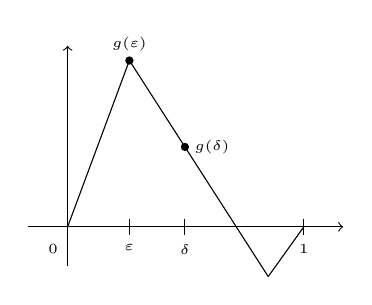
\begin{tikzpicture}
\draw[->] (0,-0.5) -- (0,2.3);
\draw[->] (-0.5,0) -- (3.5,0);
\draw[-] (0,0) --(0.78475,2.11261);
\draw[-] (0.78475,2.11261) -- (2.548,-0.631);
\draw[-] (2.548,-0.631) -- (3,0);
\fill[] (0.78475,2.11261) circle[radius=1.5pt] node[above] {\tiny $ g(\varepsilon) $};
\fill[] (0.6*0.78475+0.4*2.548,0.6*2.11261- 0.4*0.631) circle[radius=1.5pt] node[right] {\tiny $ g(\delta) $};
\draw[] (0,0.1) -- (0,-0.1) node[below left] {\tiny $ 0 $};
\draw[] (0.78475,0.1) -- (0.78475,-0.1) node[below] {\tiny $ \varepsilon $};
\draw[] (0.6*0.78475+0.4*2.548,0.1) -- (0.6*0.78475+0.4*2.548,-0.1) node[below] {\tiny $ \delta $};
\draw[] (3,0.1) -- (3,-0.1) node[below] {\tiny $ 1 $};
\end{tikzpicture} }
\captionsetup{labelformat=empty}
\caption{Illustration of the argument above. Clearly, $g([0,\varepsilon]) = g([0,\delta])$.}\label{fig:einplot}
\end{figure}

\noindent By choice of $f$, there exists at least one $H_i \neq 0$, thus, we may assume $H_1 \neq 0$. Since $\delta$ can be chosen arbitrarily small, it follows that $g'$ is not constant and hence $g$ is not constant. Hence, locally to the right of $0$, $g(x)$ is either monotonically increasing or monotonically decreasing. In the following we discuss the case where $g(x)$ is increasing, the case where $g(x)$ is decreasing can be handled analogously. It follows that there exist $\varepsilon, \delta \in (0,1)$ such that $ \varepsilon < \delta$ with the following properties: The function $g$ is increasing on $[0, \epsilon]$ with $g (\varepsilon) > 0$. On $[\varepsilon, \delta]$, $g$ is decreasing and $ 0 < g(\delta) < g(\varepsilon)$.



Using~\eqref{EqEqinDist} we infer
\begin{equation*}
g(U_{\varepsilon}) \stackrel{d}{=} B(\varepsilon, \delta) g(U_{\delta}) + A(\varepsilon, \delta).
\end{equation*}

However, by the choice of $\varepsilon$ and $\delta$, we have $g([0, \varepsilon]) = g([0, \delta])$, which immediately implies that $A(\varepsilon, \delta)=0$ and $B(\varepsilon, \delta)=1$. In the following, we use that $g(U_{\delta})$ conditioned on the event $ \left[U_{\delta} \leq \varepsilon \right] $ is in distribution equal to $ g(U_{\varepsilon}) $ and $\bbP \left[g(U_{\varepsilon}) \leq g(\delta) \right] > 0$, since $g(\delta)>0$. This leads to

\begin{multline*}
\bbP\left[g(U_{\delta}) \leq g(\delta)\right]
\\
\begin{aligned}
&= \bbP\left[g(U_{\delta}) \leq g(\delta) | U_{\delta} \leq \varepsilon \right] \bbP \left[U_{\delta} \leq \varepsilon \right] + \underbrace{\bbP\left[g(U_{\delta}) \leq g(\delta) | U_{\delta} > \varepsilon \right]}_{=0} \bbP \left[U_{\delta} > \varepsilon \right] \\
&=\bbP \left[g(U_{\varepsilon}) \leq g(\delta) \right] \bbP \left[U_{\delta} \leq \varepsilon \right] \\
&<\bbP \left[g(U_{\varepsilon}) \leq g(\delta) \right],
\end{aligned}
\end{multline*}
which is an immediate contradiction to $g(U_\varepsilon) \stackrel{d}{=} g(U_\delta)$.
\end{proof}

\begin{thebibliography}{99}
\bibitem[AS03]{all_shall} Jean-Paul Allouche and Jeffrey Shallit, \emph{Automatic Sequences. Theory, Applications, Generalizations}, Cambridge University Press, 2003.
\bibitem[RS92]{rock_sz} Andrew M. Rockett and Peter Sz\"usz, \emph{Continued fractions}, World Scientific, 1992.
\bibitem[DV86]{diamond_vaaler} Harold G. Diamond and Jeffrey D. Vaaler, ``Estimates for partial sums of continued fraction partial quotients'', \emph{Pac. J. Math.} \textbf{122} (1986), 73--82.
\bibitem[KN74]{kuipers} Lauwerens Kuipers and Harald Niederreiter, \emph{Uniform Distribution of Sequences}, Pure and Applied Mathematics, John Wiley \& Sons, 1974.
\bibitem[Her79]{herman} Michael R. Herman, ``Sur la Conjugaison Diff\'erentiable des Diff\'eomorphismes du Cercle \`a des Rotations'', \emph{Publ. Math., Inst. Hautes \'Etud. Sci.} \textbf{49} (1979), 5--233.
\bibitem[FH23]{upper_dens} Lorenz Fr\"uhwirth and Manuel Hauke, ``On the metric upper density of Birkhoff sums for irrational rotations'', \emph{Nonlinearity} \textbf{36} (2023), 7065--7104.
\bibitem[DS20]{quenched} Dmitry Dolgopyat and Omri M. Sarig, ``Quenched and annealed temporal limit theorems for circle rotations'', \emph{Some aspects of the theory of dynamical systems: a tribute to Jean-Christophe Yoccoz}, Ast\'erisque, vol. 415, Soci\'et\'e Math\'ematique de France, 2020, pp. 59--85.
\bibitem[DS41]{duff_sch} Richard J. Duffin and Albert C. Schaeffer, ``Khintchine's problem in metric Diophantine approximation'', \emph{Duke Math. J.} \textbf{8} (1941), 243--255.
\bibitem[Cas50]{cassels} John W. S. Cassels, ``Some metrical theorems in Diophantine approximation I'', \emph{Math. Proc. Camb. Philos. Soc.} \textbf{46} (1950), 209--218.
\bibitem[Bil95]{billingsley} Patrick Billingsley, \emph{Probability and measure}, 3rd ed., John Wiley \& Sons, 1995.
\end{thebibliography}
\end{document}
